\documentclass[border=3mm]{standalone}
\usepackage{tikz}
\usetikzlibrary{calc}

\begin{document}
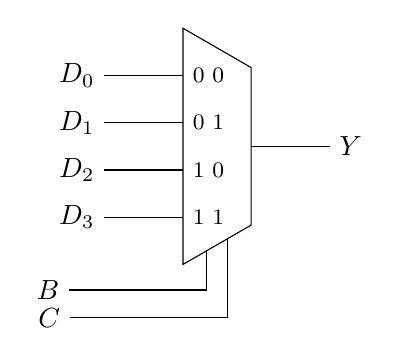
\begin{tikzpicture}
\draw (0,0)coordinate (O)--++(30:1)coordinate (A)--++(90:2)coordinate (B)--++(150:1)coordinate (C)--cycle;
\draw ($(A)!0.5!(B)$)--++(0:1)node[right]{$Y$};
\draw ($(O)!0.65!(A)$)--++(-90:1.0)--++(180:2)node[left]{$C$};
\draw ($(O)!0.35!(A)$)--++(-90:0.5)--++(180:1.75)node[left]{$B$};
%\draw ($(O)!0.75!(A)$)--++(-90:1.5)--++(180:2.25)node[left]{$c$};
%\foreach \y/\t in {0.1/1,0.2/2,0.3/3,0.4/4,0.5/5,0.6/6,0.7/7,0.8/8} {
\foreach \y/\t/\b/\c in {0.1/0/0/0,0.2/1/0/1,0.3/2/1/0,0.4/3/1/1} {
\draw ($(C)! \y*2.0 !(O)$)--++(180:1) node[left] {$D_{\t}$};
\draw ($(C)! \y*2.0 !(O)$)++(0:0.0) node[right,font=\footnotesize] {$\b$ $\c$};}
\end{tikzpicture}
\end{document}
